\chapter{Spettroscopia IR}

Quali sono i tipi di vibrazioni molecolari, quali vibrazioni sono attive
nell'IR e poi si andrà a vedere la forma delle bande e il numero onda.

In seguito verrà utilizzato l'IR per la determinazione dei composti
organici

La radiazione elettromagnetica è caratterizzata dalla lunghezza d'onda e
dalla frequenza. La lunghezza d'onda è correlata all'energia della
radiazione, tramite la legge di Plank. L'energia è inversamente
proporzionale rispetto alla lunghezza d'onda.
\[
\lambda = \frac{c}{\nu}
\]

Da queste formule, si evince che all'aumentare della lunghezza d'onda,
l'energia diminuisce.

\marginpicture*{3_001}{Radiazione elettromagnetica}

La lunghezza d'onda viene solitamente espressa come nm, mentre la
frequenza si esprime in Hz. Nella spettroscopia IR, si utilizza una
terza unità di misura, ovvero il numero d'onda.
\[
\bar{\nu} = \frac{\nu}{c} = \frac{1}{\lambda}
\]

Il numero d'onda viene definito come l'inverso del numero d'onda. Il
numero d'onda quindi ha come grandezza l'inverso di una lunghezza.
Nell'IR, si utilizza il cm\ap{-1}.

Il numero d'onda è proporzionale alla frequenza e l'energia dell'onda
elettromagnetica.

L'insieme delle radiazioni elettromagnetiche è definito come spettro
elettromagnetico. La radiazione infrarossa, si trova tra le regioni del
visibile e delle microonde. Per un chimico organico, l'intervallo si
trova tra 4000 e 400 cm\ap{-1}. Questa regione si chiama infrarosso medio.

\fullpicture*{3_002}{Regione dello spettro elettromagnetico}

La spettroscopia infrarossa è una tecnica di assorbimento, che si basa
sull'interazione della luce sulla materia. Quando un fotone infrarosso
passa energia alla molecola, questa passa dal suo stato vibrazionale
fondamentale ad uno stato vibrazionale eccitato.

L'assorbimento di energia infrarossa provoca la vibrazione della
molecola.

\halfpicture*{3_003}{Regione dell'infrarosso}

\paragraph*{Modi vibrazionali}

Sono possibili \(3N-6\) vibrazioni diverse, per una molecola non
lineare. Per una molecola lineare, i modi sono invece \(3N-5\).

Esistono due tipi di vibrazione:
\begin{itemize}
\item Stretching, o stiramento
\item Bending, o piegamento
\end{itemize}

\marginpicture*{3_004}{Moti di stretching e di bending}

Lo stretching produce una variazione della distanza interatomica, mentre
il bending produce una variazione dell'angolo di legame.

In una molecola biatomica, sono possibili solo un modo di vibrazione. Se
invece si ha una una molecola con più di due atomi, allora i moti di
bending risultano possibili.

Lo stretching può essere simmetrico o asimmetrico. Le vibrazioni
simmetriche avvengono conservando la simmetria della molecola, mentre le
vibrazioni asimmetriche avvengono con una perdita di uno o più elementi
di simmetria.

Le vibrazioni di bending possono essere differenziate in due modi:
\begin{itemize}
\item Bending simmetrico
\item Bending asimentrico
\end{itemize}

Possono essere anche classificate in base al piano di vibrazione. Si
hanno quindi vibrazioni nel piano e vibrazioni fuori dal piano.

Si identificano quindi i movimenti di:
\begin{itemize}
\item Scissor, bending simmetrico nel piano \(\delta_s\)
\item Rock, bending asimmetrico nel piano \(\rho\)
\item Twist, bending simmetrico fuori dal piano \(\tau\) o \(\delta_{\text{oop}}\)
\item Wag, bending asimmetrico fuori dal piano \(\omega\) o \(\delta_{\text{oop}}\)
\end{itemize}

I diversi tipi di vibrazione vengono indicate con diversi tipi di
lettere greche.

Per lo stretching, si usa la lettera \nu\ con un pedice, per indicare se
lo stretching è simmetrico \(\nu_{\text{s}}\) o asimmetrico \(\nu_{\text{as}}\).

Per il bending, si hanno quattro lettere; \(\delta_s\) per il scissor,
\(\rho\) per il rock, la \(\tau\) per il twist e la \(\omega\) per il
wag. Molte volte, non si fa differenza tra i bending fuori dal piano,
quindi si indica questo movimento con la lettera
\(\delta_{\text{oop}}\), che indica il bending out-of-plane (bending fuori dal piano).

Per una molecola non si vedono tutti i moti di vibrazione, in quanto  la frequenza della luce deve essere uguale alla frequenza
del moto vibrazionale.
Inoltre, il momento di dipolo deve cambiare durante la vibrazione.

È possibile anche vedere meno bene rispetto a quelle teoriche, in quanto
possono cadere fuori dal range strumentale o possono essere poco intense
o possono essere coperte da altre bande.

Altre volte è possibile vedere più bande rispetto alle bande teoriche.
Queste sono bande di combinazione, ottenute come somma di due
vibrazioni, oppure si possono avere delle bande di overtone, che sono
multipli di un determinato numero d'onda.

\section{Bande IR}

La posizione di una banda può essere calcolata con la legge di Hooke, in
modo approssimativo. Gli atomi sono approssimati ad un oscillatore
armonico. La rigidità della molla è descritta da una costante di forza
\(K\).
\[
\bar{\nu} = \frac{1}{2 \pi c} \sqrt{\frac{K}{\mu}} \qquad \mu = \frac{m_1 \cdot m_2}{m_1 + m_2}
\]

\begin{figure}[H]
    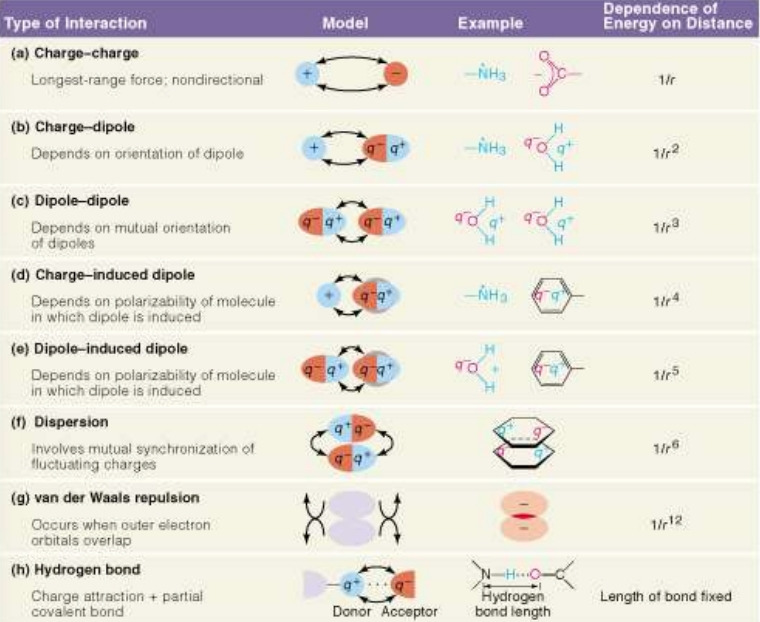
\includegraphics[width=0.9\textwidth]{3_005}
    \caption{Spettro IR}
\end{figure}

Da questa equazione, si vede che più forte è il legame e più alto è il
numero d'onda. Questo si vede nella differenza tra un legame \ce{OH},
rispetto ad un legame \ce{C-C}, quindi da una banda di stretching nell'ir a
numeri d'onda maggiori.

Da questa equazione, si vede anche che tanto maggiore è la massa degli
atomi, tanto maggiore sarà il numero d'onda.

Ci sono dei fattori chimici che alterano il valore della costante
(quindi dell'assorbimento), come il legame a idrogeno o legami intramolecolari,
effetti induttivi, effetti di risonanza, o effetti di ingombro sterico

La conseguenza è che diversi legami vibrano a diverse frequenze e
pertanto assorbono diverse frequenze IR. Quindi, la spettroscopia IR
distingue tra i diversi tipi di legami di una molecola, quindi può
essere usata per determinare i diversi gruppi funzionali della molecola.

Per quanto riguarda l'intensità delle bande IR, si deve ricordare che
nello spettro l'asse delle ordinate, si ha la trasmittanza, ovvero la
quantità di luce che passa attraverso il campione.

Una banda forte all'IR presenta un basso valore di trasmittanza, ma un
basso valore di assorbenza.

Quindi si possono distinguere le bande deboli, medie o forti. Maggiore è
il momento dipolare del legame, maggiore è l'intensità della banda.

\begin{figure}[H]
    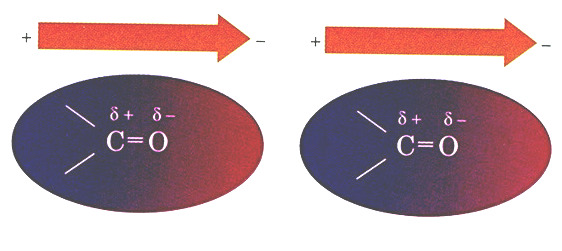
\includegraphics[width=0.5\textwidth]{3_006}
    \caption{Intensità della banda}
\end{figure}

Questo avviene perché affinché una banda sia visibile, deve variare il
momento di dipolo.

Questo si vede anche per il fatto che solitamente i gruppi funzionali
polari danno delle bande intense, mentre gruppi apolari danno bande poco
intense, o inesistenti.

La banda dipende anche dal numero di legami; se si compara lo stretching
CH dell'ottano con quello del metano, il primo è più intenso, in quanto
più legami stanno vibrando.

Come conseguenza di questo fatto, la spettroscopia IR funziona meglio
con alcuni gruppi funzionali, in particolare polari.

\subsection{Forme della banda}

La forma della banda IR è legata all'interazione del gruppo funzionale
con il suo intorno. Le bande strette indicano che il gruppo funzionale è
isolato, e che quindi non reagisce con il suo intorno.

\marginpicture*{3_007}{Forma della banda}

Se invece si vede una banda larga, il gruppo funzionale interagisce
fortemente con il suo intorno. Queste bande sono tipiche dei gruppi
funzionali che formano legami H.

\vfill
\clearpage

\section{Spettro IR}

Lo spettro IR può essere diviso in due grandi regioni
\begin{itemize}
\item Da 4000 a 1500 cm\ap{-1} si trova la regione dei gruppi funzionali
\item Da 1500 a 400 cm\ap{-1}, si trova la regione dell'impronta digitale.
\end{itemize}

La regione dei gruppi funzionali è quella più utilizzata per
diagnosticare la presenza di gruppi funzionali, in quanto sono presenti
delle bande ben visibili. Mentre per l'importo digitale è unica per ogni
molecola, però è una regione complessa e presenta un numero di bande
molto elevato. È comunque possibile ricavare dell'informazione
strutturale se si confronta con le informazioni ricavate prima, nella
regione dei gruppi funzionali

\begin{figure}[H]
    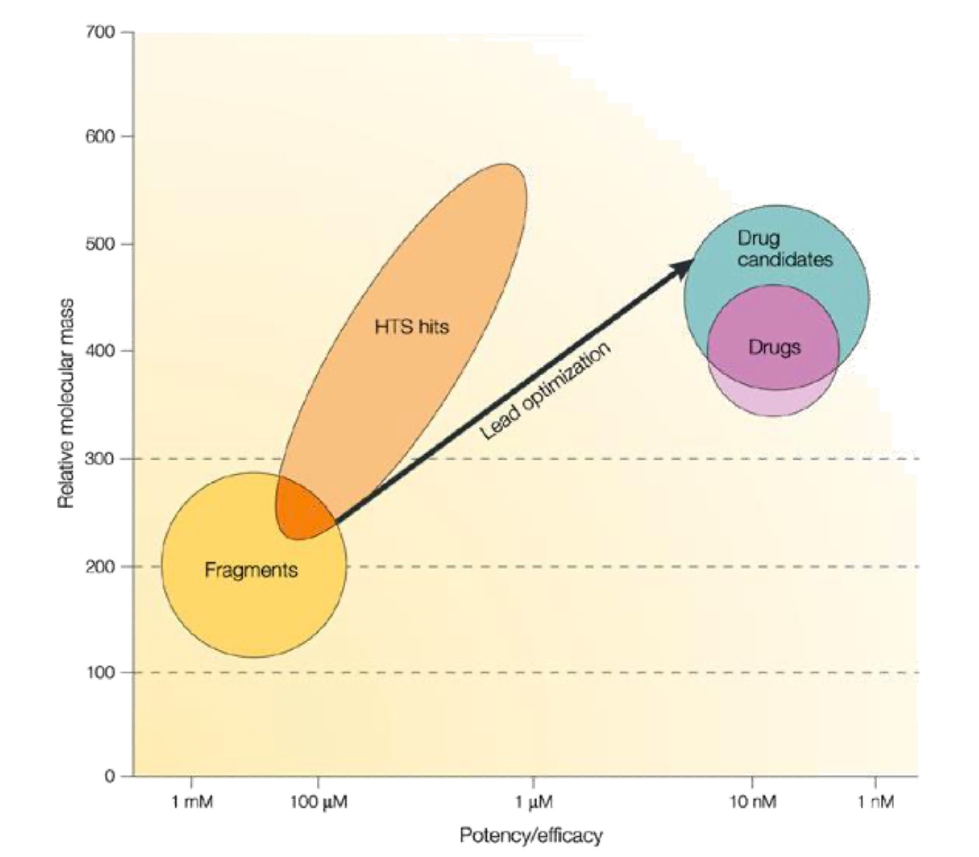
\includegraphics[width=0.9\textwidth]{3_008}
    \caption{Zone dello spettro IR}
\end{figure}

La regione dei gruppi funzionali è a sua volta divisa in tre zone:
\begin{itemize}
\item Da 4000 a 2500 cm\ap{-1}. In questa zona si vedono gli stretching dei legami con
l'idrogeno, ovvero CH, \ce{OH} o \ce{NH}.
\item La seconda zona da 2500 a 2000 cm\ap{-1}, si trovano le bande di stretching del triplo legame, quindim sia per CC, che per CN
\item Da 2000 a 1500 cm\ap{-1}, si trovano le bande diagnostiche del doppio legame CC, CO o CN.
\end{itemize}

Sotto i 1500 cm\ap{-1} si trovano gli stretching per un legame semplice e anche
tutte le vibrazioni di bending

\section{Bande diagnostiche}

Si può diagnosticare la presenza di gruppi funzionali, in base alla
presenza di alcune bande dette bande diagnostiche

\subsection{Alcani}

Il primo gruppo funzionale sono gli alcani. Sono presenti due tipi di
legame, ovvero \ce{C-H} e \ce{C-C}.

La banda diagnostica più caratteristica è la banda di stretching del
legame \ce{C-H}, che dà luogo ad una banda immediatamente sotto i 3000 cm\ap{-1}.
Questa banda è accompagnata dalle bande di bending nella zona
dell'impronta digitale. Si trovano il bending simmetrico e asimmetrico
del metile, rispettivamente a 1450 e a 1375 cm\ap{-1} e il bending simmetrico
del metilene nel piano a 1465 cm\ap{-1}. Solitamente il bending simmetrico
del metile e del metilene sono sovrapposti.

\fullpicture*{3_009}{Spettro di un alcano}

Se si tratta di un alcano a catena lunga, il metilene da un bending nel
piano del metilene a 720 cm\ap{-1}.

Ad esempio, in uno spettro dell'alcano si vede lo stretching del legame
\ce{C-H}, la banda è sotto i 3000 cm\ap{-1}.

Si trovano anche le bande di bending simmetrico del metile e del
metilene, intorno a 1450 cm\ap{-1}, e anche il bending simmetrico del metile,
intorno a 1370 cm\ap{-1}.

Lo spettro è di un alcano a catena lunga, quindi si vede anche il
bending wag a 720 cm\ap{-1}.

Si osserva che non sono state trovate le bande di stretching \ce{C-C}, o
bending \ce{C-C} o altre bande di bending (wagging o twisting) del metilene.
Queste bande di solito sono molto deboli e non compaiono nello spettro.

\fullpicture*{3_011}{Sopra: spettro del benzene. Sotto: spettro del cicloesano}

Per gli alcani ciclici, si osserva che lo stretching \ce{C-H} si sposta a
numeri d'onda più bassi. Lo stesso fenomeno si osserva per il bending
scissor per il metilene.

Infatti la banda di scissor del metilene si trova a 1468 cm\ap{-1} (per il
n-esano), mentre per il cicloesano, la stessa banding si trova a 1452
cm\ap{-1}. Via via che la dimensione dell'anello diminuisce, il numero di
onda diventa più piccolo.

I gruppi isopropile e terz-butile possono essere riconosciuti per uno
sdoppiamento del bending simmetrico del metile.

Nel caso dell'isopropile, lo sdoppiamento dà luogo a due bande a 1380 e
a 1370 cm\ap{-1}, mentre nel caso del terz-butile, le due bande appaiono a
1390 e 1370 cm\ap{-1}.

\subsection{Alcheni}

Il secondo gruppo funzionale che si andrà a vedere è il gruppo alchenico
\ce{C=C}. Negli alcheni ci sono principalmente due bande diagnostiche. La
prima banda è lo stretching del legame semplice \ce{C-H}, che può dare un
numero di bande variabile, di intensità media-alta, immediatamente sopra
i 3000 cm\ap{-1}.

La seconda banda diagnostica è lo stretching del doppio legame \ce{C=C}, che
appare nell'intervallo tra 1680 e 1640 cm\ap{-1}.

Per ricavare le informazioni strutturali, sulla sostituzione, si
utilizza lo stretching \ce{C=C}, ma anche le bande di bending fuori dal piano
del \ce{C-H}, che appaiono nella zoda tra 1000 e 650 cm\ap{-1}.

Vedendo il numero e la posizione delle bande, si riesce a capire il tipo
di sostituzione dell'alchene.

Ad esempio, un alchene monosostituito, si trova una banda di stretching
\ce{C=C} a 1640 cm\ap{-1}, accompagnata a due bande di bending fuori dal piano
(\ce{C-H}) a 990 e 910 cm\ap{-1}

Quando il doppio legame è cis (disostituito), lo stretching \ce{C=C} è a 1658
ed è accompagnato da una banda debole a 700 cm\ap{-1} dovuta al bending furo
idal piano

Se invece il doppio legame è trans (disostituito), si trova lo
stretching \ce{C=C} a 1675 cm\ap{-1}, e il bending fuori dal piano si trova a 970
cm\ap{-1}

Nel caso di un doppio legame disostituito geminale, le bande appaiono a
1650 e a 890 cm\ap{-1}.

Nel caso di un doppio legame trisostituito, si trovano le bande a 1670 e
a 815 cm\ap{-1}.

Nel caso di doppi legami completamente sostituiti, non si vede nessuna
banda di bending o di stretching \ce{C-H}, in quanto gli idrogeni non sono
presenti.

Se il doppio legame è simmetrico, non si ha la banda di stretching \ce{C=C},
poiché la simmetria impedisce la variazione di dipolo durante la
transizione e quindi la banda non è attiva nell'iR.

In queste zone si trovano delle bande di interferenza, dovute ai
composti aromatici.

\fullpicture*{3_010}{Spettro del cis-2-pentene e del trans-2-pentene}

Un esempio è il cis-2-pentene e il trans-2-pentene. Nell'isomero cis, si
vede che sono presenti le due bande diagnostiche del doppio legame,
ovvero è presente lo stretching \ce{C-H} (sopra i 3000 cm\ap{-1}), mentre lo
stretching \ce{C=C} si trova a 1669 cm\ap{-1}. Si possono vedere anche le bande
della parte alchilica: lo stretching \ce{C-H} (sp\ap{3}) poco sotto i 3000,
accompagnate dai benging specifici dei metili e dei metileni (a \(\sim\)
1400 cm\ap{-1}). Inoltre, analizzando sia la posizione dello stretching \ce{C=C}
sia la regione del bending fuori dal piano del \ce{C-H}, si può vedere che si
tratta di un doppio legame cis disostituito.

Nello spettro dell'isomero trans, si vedono gli stessi picchi
diagnostici dell'isomero cis, quindi si vedono lo streching del carbonio
sp\ap{2}, sopra i 3000 cm\ap{-1} e lo streching del legame \ce{C=C} a 1874 cm\ap{-1}. Si
vede la differenza di intensità tra l'isomero cis e l'isomero trans
proprio per questo picco, la differenza di deve al momento dipolare.

Il doppio legame trans è più simmetrico e dà luogo ad una variazione del
momento dipolare, quindi la banda è più piccola.

Si vede che è l'isomero trans è sostituito, in quanto nella zona del
bending fuori dal piano si vede solo una banda, che però si è spostata a
966 cm\ap{-1}.

\subsection{Alchini}

Gli alchini daranno uno stretching del triplo legame \ce{C#C}, che si
trova ad una banda stretta, di intensità media a 2150 cm\ap{-1}. Se il triplo
legame è simmetrico, la banda è assente, perché lo stretching di un
alchino simmetrico non porta alla variazione del momento dipolare.

Un'altra banda molto importante, nel caso di un alchino terminale è lo
stretching del carbonio sp con l'idrogeno \ce{C-H}, che dà luogo ad una banda
molto intensa e molto stretta a 3300 cm\ap{-1}.

\fullpicture{3_011}{Sopra: spettro dell 1-esino. Sotto: spettro del 4-ottino}{fig:spettrialchini}

Negli esempi in figura \ref{fig:spettrialchini}, si vede che lo spettro del 1-esino, si vede che sono
presenti le due bande diagnostiche. Si vede quindi lo stretching del
triplo legame \ce{C#C} con una banda stretta a 2150 cm\ap{-1}, e si vede
anche lo stretching \ce{C-H} del carbonio sp, che dà una banda forte a 3300
cm\ap{-1}. Si vede anche tutta la parte alifatica, che si può notare nel
picco dovuto allo stretching sp\ap{3} \ce{C-H}, immediatamente sotto i 3000 cm\ap{-1}.

Nel secondo esempio, ovvero lo spettro del 4-ottino, che è un composto
simmetrico. Per via della simmetria, lo stretching del triplo legame
\ce{C#C} è assente nello spettro, perché la transizione non produce una
variazione del momento dipolare. L'alchino non è terminale e quindi non
si vede neanche lo stretching del carbonio sp con l'idrogeno \ce{C-H}.

Con questo, si vuole dire che anche se non si vede lo stretching del
legame \ce{C#C} o del doppio legame \ce{C=C}, non significa che il gruppo
funzionale sia presente. Bisogna confrontare i dati con gli spettri NMR
per capire effettivamente cosa è presente.

\subsection{Aromatici}

I composti aromatici sono alla fin fine composti con dei doppi legami,
che però sono coniugati, quindi ci si aspetta di vedere le stesse bande
diagnostiche per un doppio legame.

Infatti, le bande diagnostiche per gli aromatici sono lo stretching del
carbonio sp\ap{2} con l'idrogeno (\ce{C-H}), che appare appena sopra i 3000 cm\ap{-1},
lo stretching del doppio legame \ce{C=C}, che dà luogo a due bande per gli
aromatici, una a 1605 cm\ap{-1} e una a 1475 cm\ap{-1}.

Si hanno anche le bande di bending fuori dal piano del legame \ce{C-H}, che
vanno da 900 a 690 cm\ap{-1}.

Per gli aromatici, si hanno anche delle bande di combinazione, che sono
bande normalmente deboli, che appaiono da 2000 a 1667 cm\ap{-1}.

Per ricavare informazioni sulla sostituzione dell'anello, si va ad
analizzare le due regioni delle bande di combinazione e del bending CH
fuori dal piano.

Per quanto riguarda le bande di combinazione, sono bande deboli, a volte
non si vedono. Inoltre è possibile avere delle interferenze con altri
gruppi funzionali come il carbonile. Se si possono vedere, aiutano a
capire la sostituzione dell'anello, poiché ogni tipo di sostituzione dà
luogo a un numero di bande e a un profilo ben diverso.
\fullpicture*{3_012}{Informazioni strutturali di un composto aromatico}

Questa informazione deve essere analizzata insieme alla zona del bending
CH fuori dal piano, quindi tra 900 e 690 cm\ap{-1}. Un composto aromatico
monosostituito presenta un profilo di combinazione con cinque segnali;
questo profilo però sarà accompagnato da due bande intense tra 800 e 600
cm\ap{-1}.

Se invece si ha un composto disostituito in orto, si vedrà il
corrispondente profilo per le bande di combinazione che sarà
accompagnato da una sola banda intorno a 750 cm\ap{-1}, per il bending fuori
dal piano

Nel caso del meta, invece si avrà il profilo caratteristico delle bande
di combinazione, mentre si avranno due bande intense tra 800 e 650 cm\ap{-1}.

Si può quindi ottenere informazione strutturale per i diversi tipi di
sostituzione.

\fullpicture*{3_013}{Spettri del toluene e del meta-xilene}

Come esempio, sono presenti gli spettri del toluene e del m-xilene. In
tutti e due si vedono le bande diagnostiche dei composti aromatici,
ovvero gli stretching del carbonio sp\ap{2} con l'idrogeno \ce{C-H},
immediatamente sopra i 3000 cm\ap{-1}, ed in entrambi, si vedono le due bande
tipiche del doppio legame \ce{C=C} degli aromatici, a 1605 e 1496 cm\ap{-1}, per
il toluene e a 1614 cm\ap{-1} e a 1492 cm\ap{-1} per il m-xilene.

Inoltre, si vedono le bande di combinazione. Se si analizza il profilo e
il numero delle bande di combinazione, insieme alla regione del bending
fuori dal piano, si arriva alla conclusione che un profilo appartiene a
un composto monosostituito, mentre nel caso del m-xilene, si può
osservare che il profilo delle due regioni appartiene ad un composto in
meta.

\fullpicture*{3_014}{Spettri del para-xilene e del orto-xilene}

Si vedono anche gli spettri del p-xilene e del o-xilene, dove sono
presenti le bande diagnostiche per i composti aromatici, ovvero lo
stretching \ce{C-H} sopra i 3000 cm\ap{-1} e le due bande di stretching del legame
\ce{C=C} a 1630 cm\ap{-1}.

Si vedono anche le bande di combinazione e le bande del bending fuori
dal piano, che identificano un composto in rispettivamente sostituito in
para e in orto.

\paragraph*{Aromatico contro alchene}

Sicuramente, il grado di insaturazione dà un'indicazione del numero di
insaturazioni presenti.

Il grado di insaturazione determina la somma del numero di cicli, dei
doppi legami e il doppio del numero dei tripli legami

Il grado di insaturazione può essere calcolato con la formula
\[
\text{I} = \text{C} - \frac{\text{H}}{2} - \frac{\text{X}}{2} + \frac{\text{N}}{2} + 1
\]

Rispettivamente, si vanno a calcolare il numero di atomi tetravalenti
(C), metà del numero di atomi monovalenti (H e X) e metà del numero di
atomi trivalenti.

Il grado di insaturazione del benzene è di quattro (tre doppi legami ed
un ciclo), che è molto elevato per una molecola formata da sei atomi di
carbonio.

In secondo luogo, gli aromatici hanno delle bande di combinazione tra
2000 e 1667 cm\ap{-1}, che sono assenti negli alcheni.

Gli aromatici, inoltre, presentano una banda a 1605 cm\ap{-1}, per via dello
stretching \ce{C=C}.

Infine, l'intensità per lo stretching \ce{C=C} è più grande per un aromatico,
rispetto ad un alchene.

\subsection{Alcoli}

Questi due gruppi hanno uno stretching eteroatom\ce{OH} nella zona tra 3600
a 3000 cm\ap{-1}. Lo stretching \ce{OH} sarà comune a alcoli e acidi carbossilici,
mentre lo stretching N-H si ritroverà nelle ammine e nelle ammidi.

Si può riconoscere le ammidi e gli acidi carbossilici in base allo
stretching del \ce{C=O}. Bisogna fare attenzione ad altre interferenze
presenti, come lo stretching di alchini terminali e di alcheni.

Un altra molecola che interferisce in questa zona è l'acqua, l'acqua dà
una banda forte di stretching \ce{OH} in questa zona.

Ogni interpretazione fatta sullo spettro IR deve essere logica, cioè non
si può assegnare uno stretching \ce{OH} se nella formula bruta non sono
presenti atomi di ossigeno. Allo stesso modo, non si può assegnare un
picco di un alchino terminale, se il grado di insaturazione non è minimo
due.

Per gli alcoli, si vedono due stretching caratteristici:
\begin{itemize}
\item Stretching \ce{OH}
nella zona tra 3600 e 3200 cm\ap{-1}, che dà una banda larga e intensa. La
forma e la posizione dipende fortemente dalla possibilità di formare
legami ad idrogeno.
\item Stretching \ce{C-O}, si vede nella zona tra 1300 e 1000
cm\ap{-1}. La banda è intensa e più stretta. Questa banda si trova anche
negli eteri
\end{itemize}

La seconda banda può dare informazioni strutturali.

Il primo stretching \ce{OH} dipende dalla possibilità di formare legami H.
Questo perché i ponti a idrogeno indeboliscono il legame \ce{OH},
facilitando lo stiramento. La banda quindi si allarga e si sposta a
numeri d'onda minori.

Ad esempio, per alcoli, fenoli e acidi carbossilici, si osserva che in
assenza di ponti ad idrogeno, la banda \ce{OH} appare come una banda tra 3650
e 3590 cm\ap{-1}. È una banda stretta, in quanto non interagisce con il suo
intorno.

Invece, in presenza di ponti a idrogeno intermolecolari, la banda si
allarga e si sposta fino a 3200 cm\ap{-1}. Se invece i ponti a idrogeno sono
intramolecolari, la banda si sposta in un range da 3200 a 2500 cm\ap{-1}.

\marginpicture{3_015}{Effetti della concentrazione e del solvente}{fig:concalcoli}


Nella figura \ref{fig:concalcoli}, ci sono due esempi dell'effetto del legame a idrogeno.
Nella figura a, si ha uno spettro IR, con la banda dello stretching \ce{OH},
per una soluzione di alcol in tetracloruro di carbonio a diverse
concentrazioni. In una soluzione molto diluita, si osserva soltanto lo
stretching \ce{OH} isolato a 3600 cm\ap{-1}.
Man mano che aumenta la concentrazione, la banda si allarga e si sposta
a destra, in quanto ad alte concentrazioni si favorisce la formazione
del legame a idrogeno intermolecolare.
Nella figura b invece si vede l'effetto del solvente. La zona è sempre
quella dello stretching \ce{OH}; la concentrazione rimane costante, ma cambia
il solvente.

Si vede che la banda dello stretching \ce{OH} è localizzata a 3600 cm\ap{-1}
quando il solvente non può formare legami ad idrogeno (come nel
benzene); si vede una banda stretta.
Se invece il solvente può formare legami H, si vede che la banda si
sposta a destra e si allarga in quanto si forma legame a idrogeno tra l'alcol e
il solvente.
Questo effetto del legame a idrogeno, si vede anche a seconda delle condizioni di
registro dello spettro IR.

\fullpicture*{3_016}{Spettro di un alcol registrato in fase gas, in una soluzione di \ce{CCl4} e in film}

Se l'IR è registrato in fase gas, non c'è legame a idrogeno, mentre se si fa in
una soluzione diluita in \ce{CCl4}, si vede lo stretching \ce{OH} isolato a 3600
cm\ap{-1}, ma anche si vede l'ossidrile impiegato nella formazione del legame
H a 3340 cm\ap{-1}. Quando invece si registra il composto in un film (composto puro non
diluito), si vede la banda dello stretching \ce{OH} che forma il legame a idrogeno a
3324 cm\ap{-1}.

\fullpicture*{3_017}{Stretching \ce{C-O}, che descrive le informazioni strutturali dell'alcol}

Lo stretching \ce{C-O} è meglio descrivibile come stretching \ce{C-C-O}, in quanto
le due vibrazioni accoppiano tra loro e danno una banda tra 1300 e 1000 cm\ap{-1}.

Questa banda è intensa e più o meno stretta; si trova anche negli eteri,
che però prende il nome di banda \ce{C-O-C}.
Questa banda dà informazioni strutturali sul tipo di alcol o di etere.

Per gli alcoli primari, lo stretching \ce{C-O} dà una banda a 1050 cm\ap{-1}, che
si sposta a 1100 cm\ap{-1} per alcoli secondari, 1150 cm\ap{-1} per alcoli
terziari e a 1220 cm\ap{-1} per alcoli aromatici (fenoli)

Per quanto riguarda gli eteri, la banda dà informazioni sulla simmetria
dell'etere. Gli eteri dialchilici simmetrici danno una sola banda
intorno a 1125 cm\ap{-1}. Mentre gli eteri asimmetrici danno di solito due bande:
\begin{itemize}
\item Se si tratta di un aril alchil etere, si avranno due bande a 1250 e a 1040 cm\ap{-1}
\item Se si tratta di un vinil alchil etere, si avranno due bande a 1220 e a 850
cm\ap{-1}.
\end{itemize}

Un esempio è lo spettro dell'etere etilico, in figura \ref{fig:spettroetere}. In questo spettro, si vede
che si riesce ad identificare facilmente lo stretching del carbonio sp\ap{3} - H, corrispondente alla parte alifatica. Si riesce anche a vedere il
bending della fase alifatica.

Nella zona dell'impronta digitale si vede una banda intensa, che è lo
stretching del legame singolo \ce{C-O}, che identifica l'etere.

Nel secondo esempio, c'è lo spettro dell'anisolo che è un aril alchil
etere. Si vedono i segnali diagnostici del benzene, che corrispondono
alle bande sopra 3000 cm\ap{-1}, le bande sono di stretching \ce{C-H}. Si vedono
anche le bande di combinazione e anche le bande del doppio legame a 1600
e a 1498 cm\ap{-1}.

Nella zona dell'impronta digitale, si vedono varie bande. Le più forti
sono quelle dello stretching \ce{C-O}. Le bande sono due, quindi l'etere è
asimmetrico.

In questi due esempi si vede che è difficile identificare un etere dal
solo spettro IR, è meglio usare l'NMR.

\begin{figure}[H]
    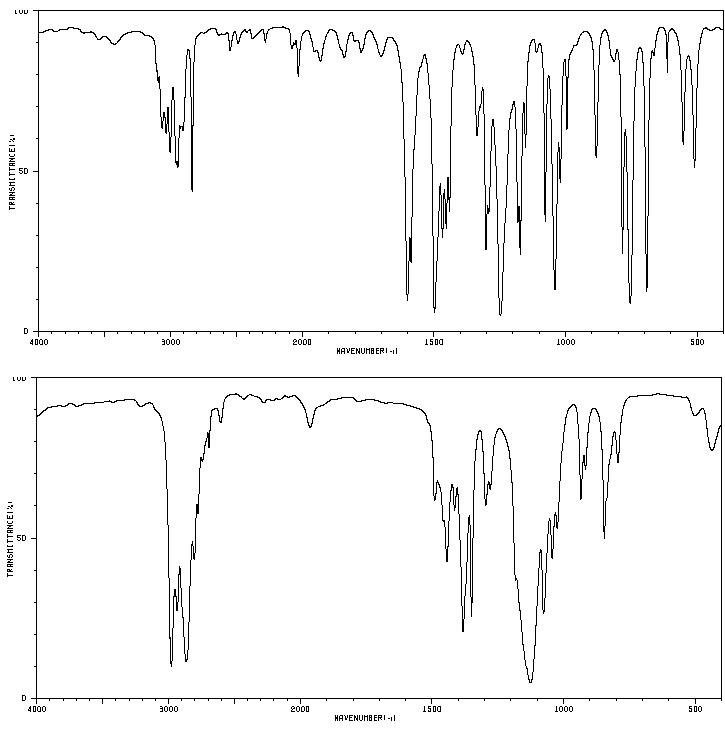
\includegraphics[width=0.9\textwidth]{3_018}
    \caption{Sopra: spettro dell etere etilico. Sotto: spettro del anisolo}
    \label{fig:spettroetere}
\end{figure}

\vfill

\subsection{Ammine}

Le ammine hanno anch'esse una banda nella zona tra 3600 e 3200 cm\ap{-1}.
Questa banda corrisponde allo stretching \ce{OH}.

Le ammine primarie danno due bande in questa zona, ovvero a \(\sim\)
3500 e a \(\sim\) 3400 cm\ap{-1}. Queste due bande di intensità media,
saranno accompagnate da una banda di bending che compare tra 1650 e 1580
cm\ap{-1}, con un'intensità forte. Le ammine secondarie danno un solo stretching NH tra 3350 e 3310 cm\ap{-1}.
Le ammine terziarie non danno luogo ad nessun stretching NH.

La seconda banda caratteristica è data dallo stretching C-N. In realtà
questa banda è poco utile, perché è presente nella zona dell'impronta
digitale e ha un'intensità medio-debole, e quindi è difficile da
individuare.

Le ammine alifatiche danno una banda intorno a 1250 e 1020 cm\ap{-1}, mentre
le ammine aromatiche danno luogo ad una banda tra 1340 e 1266 cm\ap{-1}. Nel
secondo caso, la banda è abbastanza forte.

\begin{figure}[H]
    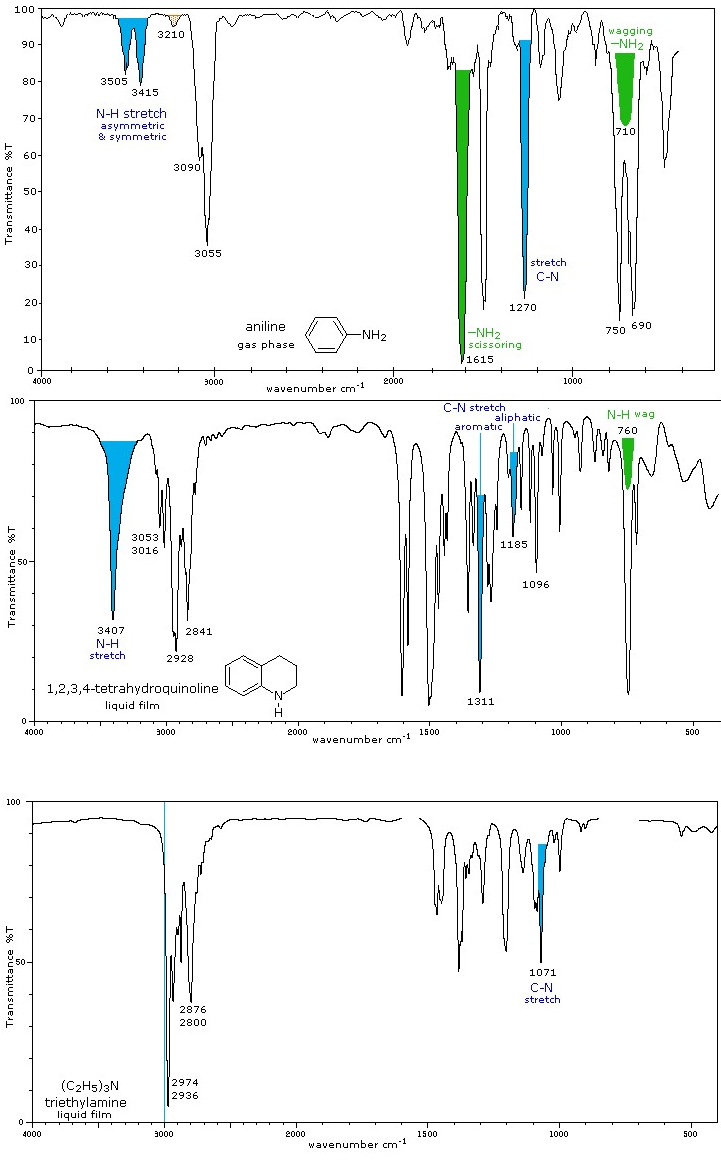
\includegraphics[width=0.68\textwidth]{3_019}
    \caption{Spettri IR di un ammina primaria, secondaria e terziaria}
\end{figure}

Sono riportati tre esempi di queste tre ammine, una aromatica, una
secondaria e la trietilammina (ammina alifatica).

Per l'ammina primaria si vedono i due stretching NH a 3500 e 3415 cm\ap{-1},
per l'ammina secondaria aromatica, si vede un solo stretching NH, mentre
per un'ammina terziaria non si vede lo stretching \ce{NH}.

Per l'ammina primaria, si vede anche il bending \ce{NH2} intorno a 1615 cm\ap{-1},
con una banda molto forte. Si vede anche lo stretching del legame C-N,
con una banda a 1270 cm\ap{-1}.

Per l'ammina secondaria aromatica, è più difficile individuare lo
stretching C-N; si hanno due stretching, uno a 1185 cm\ap{-1} che è quello
del carbonio alifatico con l'azoto e l'altro a 1311 cm\ap{-1}, più forte, che
è quello dello stretching carbonio aromatico-azoto.

Per un'ammina terziaria alifatica, si vede che c'è lo stretching C-N a
1071 cm\ap{-1}, però è debole.

Quindi per le ammine, si individua bene lo stretching NH e nel caso
dell'ammina primaria, si può vedere bene il bending NH2. Però bisogna
fare attenzione perché in questa zona sono presenti anche gli stretching
del doppio legame \ce{C=C}.

\subsection{Carbonile}

Questo gruppo funzionale è quello che è più facilmente riconoscibile
nella spettroscopia IR. Questo gruppo dà una banda di stretching \ce{C=O}
intorno a 1700 cm\ap{-1}, che normalmente è la banda più intensa dello spettro.

La posizione di questa banda dipende dalla funzionalizzazione, e questo
permette di differenziare il gruppo carbonile nei diversi gruppi
funzionali.

Come si vede, un cloruro acilico ha lo stretching \ce{C=O} a 1807 cm\ap{-1}. Per
gli anidridi, si hanno due bande, una a 1832 cm\ap{-1} e una a 1761 cm\ap{-1}.
Gli esteri invece danno una banda del carbonile a 1740 cm\ap{-1}. Le aldeidi
a 1730 cm\ap{-1} e i chetoni a 1715 cm\ap{-1}.
Gli acidi carbossilici, di solito si vedono a 1700 cm\ap{-1}, che corrisponde
alla forma dimerica dell'acido carbossilico. La forma monomerica appare
a 1760 cm\ap{-1}, anche se di solito non si vede.
Le ammidi e i chetoni coniugati hanno lo stretching \ce{C=O} sotto i 1700
cm\ap{-1}, di solito intorno a 1670 e 1680 cm\ap{-1}.

Il gruppo carbonile è importante per poter differenziare i gruppi
funzionali. Inoltre, bisogna controllare diverse zone dello spettro IR.
Ad esempio, se si sospetta di avere un estere, bisogna controllare anche
le due bande di stretching del \ce{C-O}, che sono a tra 1300 e 1000 cm\ap{-1}.
Se invece, si pensa di avere un aldeide, bisogna controllare le bande di
stretching \ce{C-H} (delle aldeidi). Lo stretching \ce{C-H} aldeidico dà due bande
di intensità media, tra 2700 e 2850 cm\ap{-1}.

Per gli acidi carbossilici, si guarda lo stretching \ce{OH}, tra 3300 e 3000
cm\ap{-1}, che sarà molto larga e dovrebbe vedersi lo stretching del legame
singolo \ce{C-O} tra 1300 e 1000 cm\ap{-1}.
Nel caso delle ammidi, bisogna vedere lo stretching N-H a 3200 cm\ap{-1}, e
anche lo stretching del legame singolo C-N
In ultimo, se si ha il sospetto di avere un chetone coniugato, bisogna
guardare anche lo stretching del legame \ce{C=C}.

\paragraph*{Stretching di \ce{C=O}}

La risposta è
in quanto il carbonile subisce gli effetti della risonanza e
dell'induzione elettronica.
Come esempio, è stato riportato il caso degli esteri e delle ammidi. In
entrambi i casi, è possibile avere un effetto di induzione e un effetto
di risonanza.

L'effetto induttivo predomina negli esteri, in quanto si ha un
eteroatomo più elettronegativo del carbonio che attira a sé la densità
elettronica e riduce il legame \ce{C=O}, quindi l'intensità è maggiore e il
segnale si sposta a numeri d'onda più alti.

Invece, per le ammidi predomina l'effetto di risonanza. I due elettroni
di non legame dell'azoto si delocalizzano, per dare una seconda forma di
risonanza. Questa forma di risonanza fa perdere intensità al legame
carbonilico. Lo stretching si sposta a numeri d'onda più bassi.

Come primo esempio di questi composti, come riportato nella figura \ref{fig:ciclochet}, sono riportati gli spettri del
cicloesanone e del della butirraldeide.

\fullpicture{3_020}{Spettri di un aldeide e di un chetone ciclico}{fig:ciclochet}

In tutti e due si vede che la banda più intensa dello spettro è intorno
a 1700 cm\ap{-1}, che rappresenta lo stretching del carbonile. Questa banda è
spostata a numeri d'onda più bassi nel chetone, in quanto la
sostituzione dell'idrogeno con un gruppo alchilico, che ha un effetto
induttivo, aumenta la lunghezza del legame \ce{C=O}, pertanto lo indebolisce.

La seconda cosa da notare è che l'aldeide ha una seconda banda
diagnostica, ovvero la banda di stretching \ce{C-H} aldeidico, che dà due
bande di intensità media-bassa a 2827 e 2725 cm\ap{-1}.

\fullpicture{3_021}{Spettro IR dell'acetofenone}{fig:acetofenone}

In un secondo esempio, in figura \ref{fig:acetofenone} invece, si ha lo spettro del cicloesanone,
però il secondo spettro è del acetofenone, che è un chetone coniugato.
Come si vede, lo stretching del carbonile si è spostato a 1716 cm\ap{-1} a
1686 cm\ap{-1}. Questo è un effetto della coniugazione, che indebolisce il
legame \ce{C=O}.

Lo stretching \ce{C=O} dipende anche dalla dimensione del ciclo. Nei chetoni
ciclici, si vede che più piccolo è il ciclo e maggiore è il numero
d'onda dello stretching \ce{C=O}. Si passa da 1716 cm\ap{-1} per il cicloesanone a
1747 cm\ap{-1} per il ciclopentanone e 1793 per il ciclobutanone.

\begin{figure}[H]
    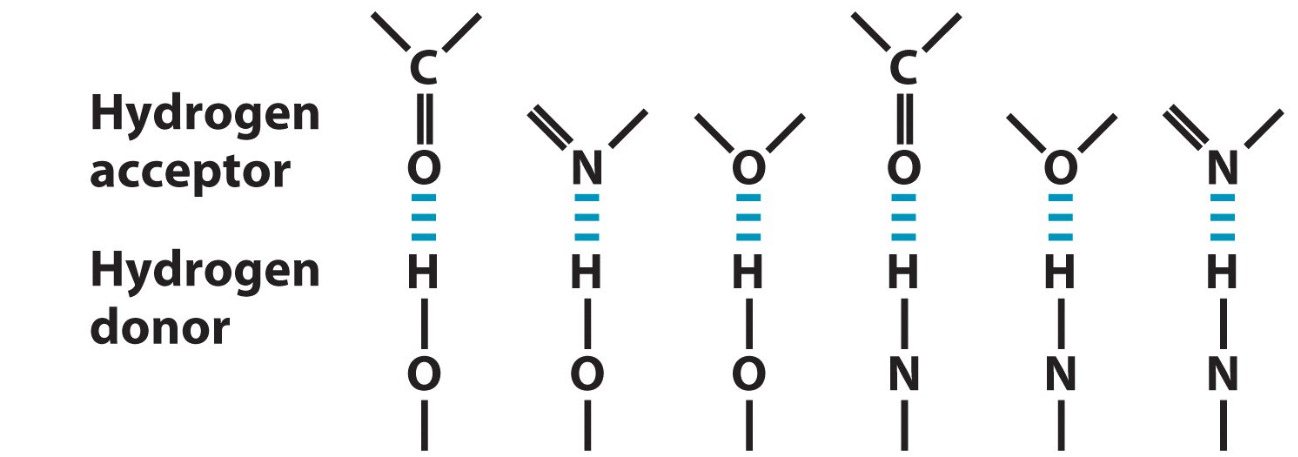
\includegraphics[width=0.8\textwidth]{3_022}
    \caption{Sopra: spettro della salicilaldeide. Sotto: spettro della benzaleide}
    \label{fig:IRald}
\end{figure}


Anche il legame a idrogeno ha un effetto sullo stretching del gruppo
carbonile. Prendendo la salicilaldeide e la benzaldeide in figura \ref{fig:IRald}, si vede che lo
stretching \ce{C=O} si sposta a numeri d'onda minori, quando c'è il legame a idrogeno.
Questo è per l'effetto del legame a idrogeno intermolecolare.

\paragraph{Acido carbossilico}

Lo spettro di un acido carbossilico prevede due bande diagnostiche,
ovvero lo stretching \ce{OH} e lo stretching del carbonile.

\fullpicture*{3_024}{Spettro di un acido carbossilico}

Lo stretching \ce{OH} è molto particolare, infatti è una banda larga e
intensa e va da 3300 cm\ap{-1} a 2500 cm\ap{-1}. Non è una banda regolare, ma
presenta dei picchi al suo interno.

Lo stretching \ce{C=O} per acidi carbossilici alifatici (non coniugati) è
intorno a 1700 cm\ap{-1}.

\paragraph{Esteri}

Negli esteri c'è sicuramente lo stretching del carbonile, sui 1740 cm\ap{-1},
per un estere alifatico non coniugato, che si sposta a numeri d'onda più
bassi per un estere coniugato.

\begin{figure}[H]
    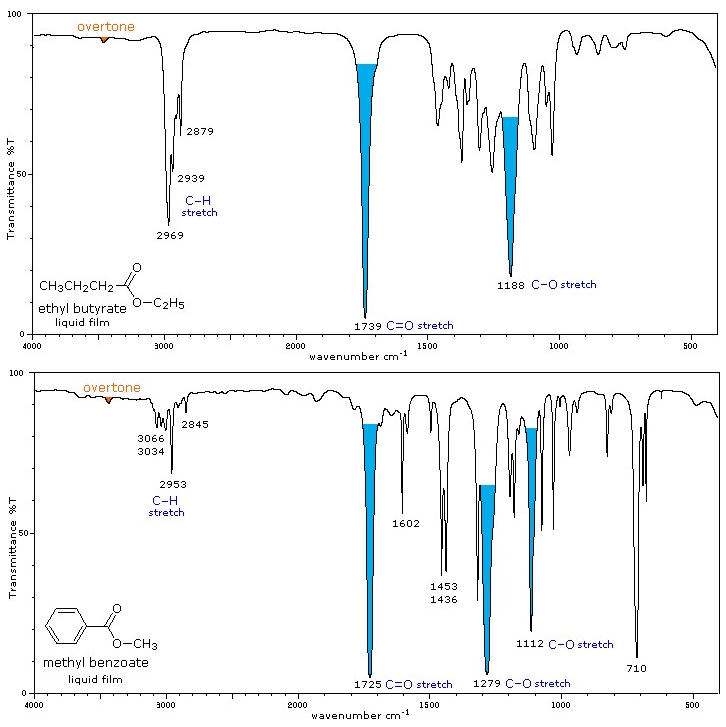
\includegraphics[width=0.8\textwidth]{3_025}
    \caption{Spettro di due esteri}
\end{figure}

Nella zona dell'impronta digitale, si hanno anche lo stretching del
legame singolo \ce{C-O}, che saranno una o più bande strette ed intense.

Per differenziare gli esteri dagli acidi carbossilici, è necessario guardare lo stretching \ce{OH}.
Gli esteri non hanno lo stretching \ce{OH} degli acidi carbossilici; inoltre,
gli esteri hanno una posizione diversa per lo stretching \ce{C=O}. È 1710
cm\ap{-1} per acidi non coniugati, e 1740 cm\ap{-1} per esteri alifatici non
coniugati

\paragraph{Ammidi}

Le ammidi hanno un segnale diagnostico, ovvero lo stretching N-H, tra
3500 e 3000 cm\ap{-1}. Quindi si vedono due stretching NH per ammidi
primarie, uno solo per ammidi secondarie e nessun segnale per le ammidi
terziarie.

Le bande si allargano in presenza di legame a idrogeno.
Si ha anche lo stretching del carbonile, che è sempre più basso di 1700
cm\ap{-1}. Questo stretching è chiamato banda ammidica I.
Si ha anche un'altra banda, questa volta di bending N-H, che è un altra
banda intensa e si trova intorno a 1600 cm\ap{-1}. Questa banda si chiama
banda ammidica II.

Nella zona dell'impronta digitale, si trova anche lo stretching del
legame singolo C-N, che è una banda intorno a 1400 cm\ap{-1}.

\begin{figure}[H]
    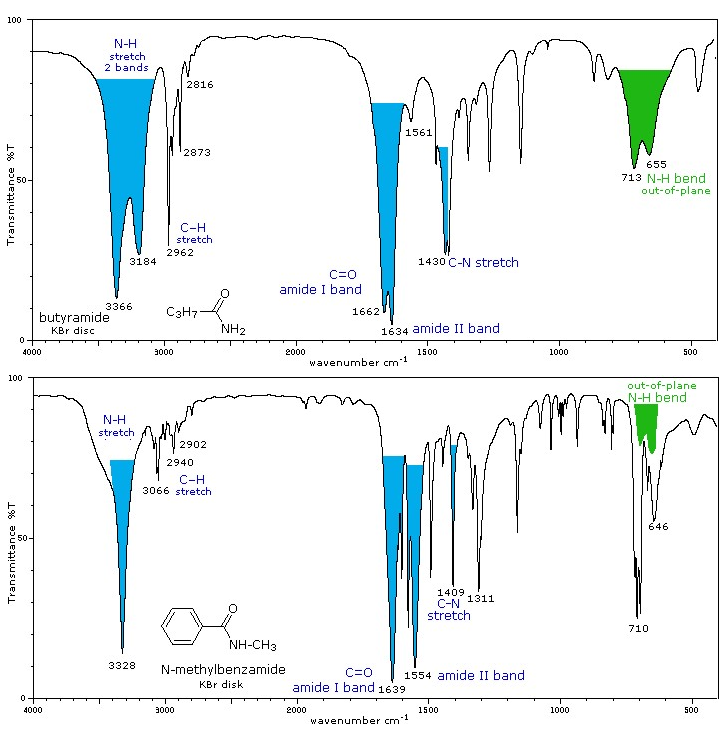
\includegraphics[width=0.8\textwidth]{3_026}
    \caption{Spettro di due ammidi}
\end{figure}

Per un ammide alifatica primaria, si vede come segnale diagnostico, i
due stretching \ce{N-H}, sopra i 3000 cm\ap{-1}. Si vede anche lo stretching del
carbonile, a 1642 ed anche il bending del \ce{NH2}.

Per un ammide coniugata secondaria, si vede lo stretching \ce{N-H}, sopra i
3000 cm\ap{-1}, con una sola banda. Si vede anche lo stretching \ce{C=O}, che però
si è spostato a numero d'onda minori, se comparato a quello sopra.
Questo avviene in quanto c'è coniugazione.

Si vede inoltre il bending dell'\ce{N-H}; anche questo segnale si è spostato
in seguito alla coniugazione.

\fullpicture*{3_023}{Posizione del gruppo funzionale carbonile, a seconda del composto}

\paragraph{Nitrilo}

Il nitrilo possiede un triplo legame \ce{C#N}, che dà una banda
caratteristica (forte e stretta) tra 2200 e 2300 cm\ap{-1}.

\paragraph{Nitro}

Il gruppo nitro dà due bande forti a 1550 cm\ap{-1} e l'altra a 1370 cm\ap{-1}.

\paragraph{Tioli}

I tioli danno una banda di stretching SH che è molto debole, però appare
in una posizione isolata, quindi può essere utilizzata. La banda si
trova a 2600 cm\ap{-1}.

\paragraph{Promemoria}
I gruppi \ce{OH} e \ce{NH} sono presenti in molti composti, tra 3400 e 3000 cm\ap{-1}. Come
si identificano?

\begin{figure}[H]
    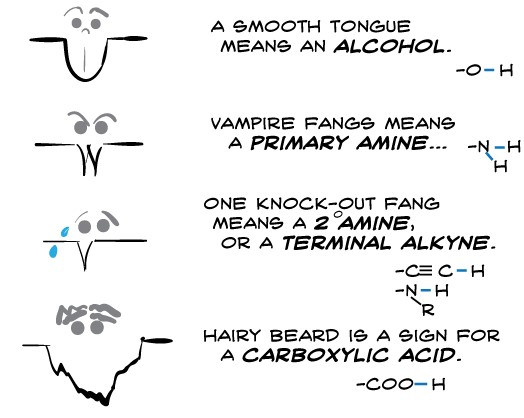
\includegraphics[width=0.5\textwidth]{3_027}
    \caption{Forma delle bande dei gruppi \ce{OH} e \ce{NH}}
\end{figure}

Se la forma della banda è liscia, si tratta di un alcol. Se invece le
bande formano delle zanne, si tratta di un ammina o un ammide primaria.
Se invece la forma della banda ricorda un solo dente, si ha un ammina o
ammide secondaria, o un alchino terminale.
Se invece si ha una forma simile ad una barba, si tratta di un acido
carbossilico.

\vfill

\begingroup
\checkoddpage
\makebox[\textwidth][\ifoddpage r\else l\fi]{\kern-\csname Gm@\ifoddpage l\else r\fi margin\endcsname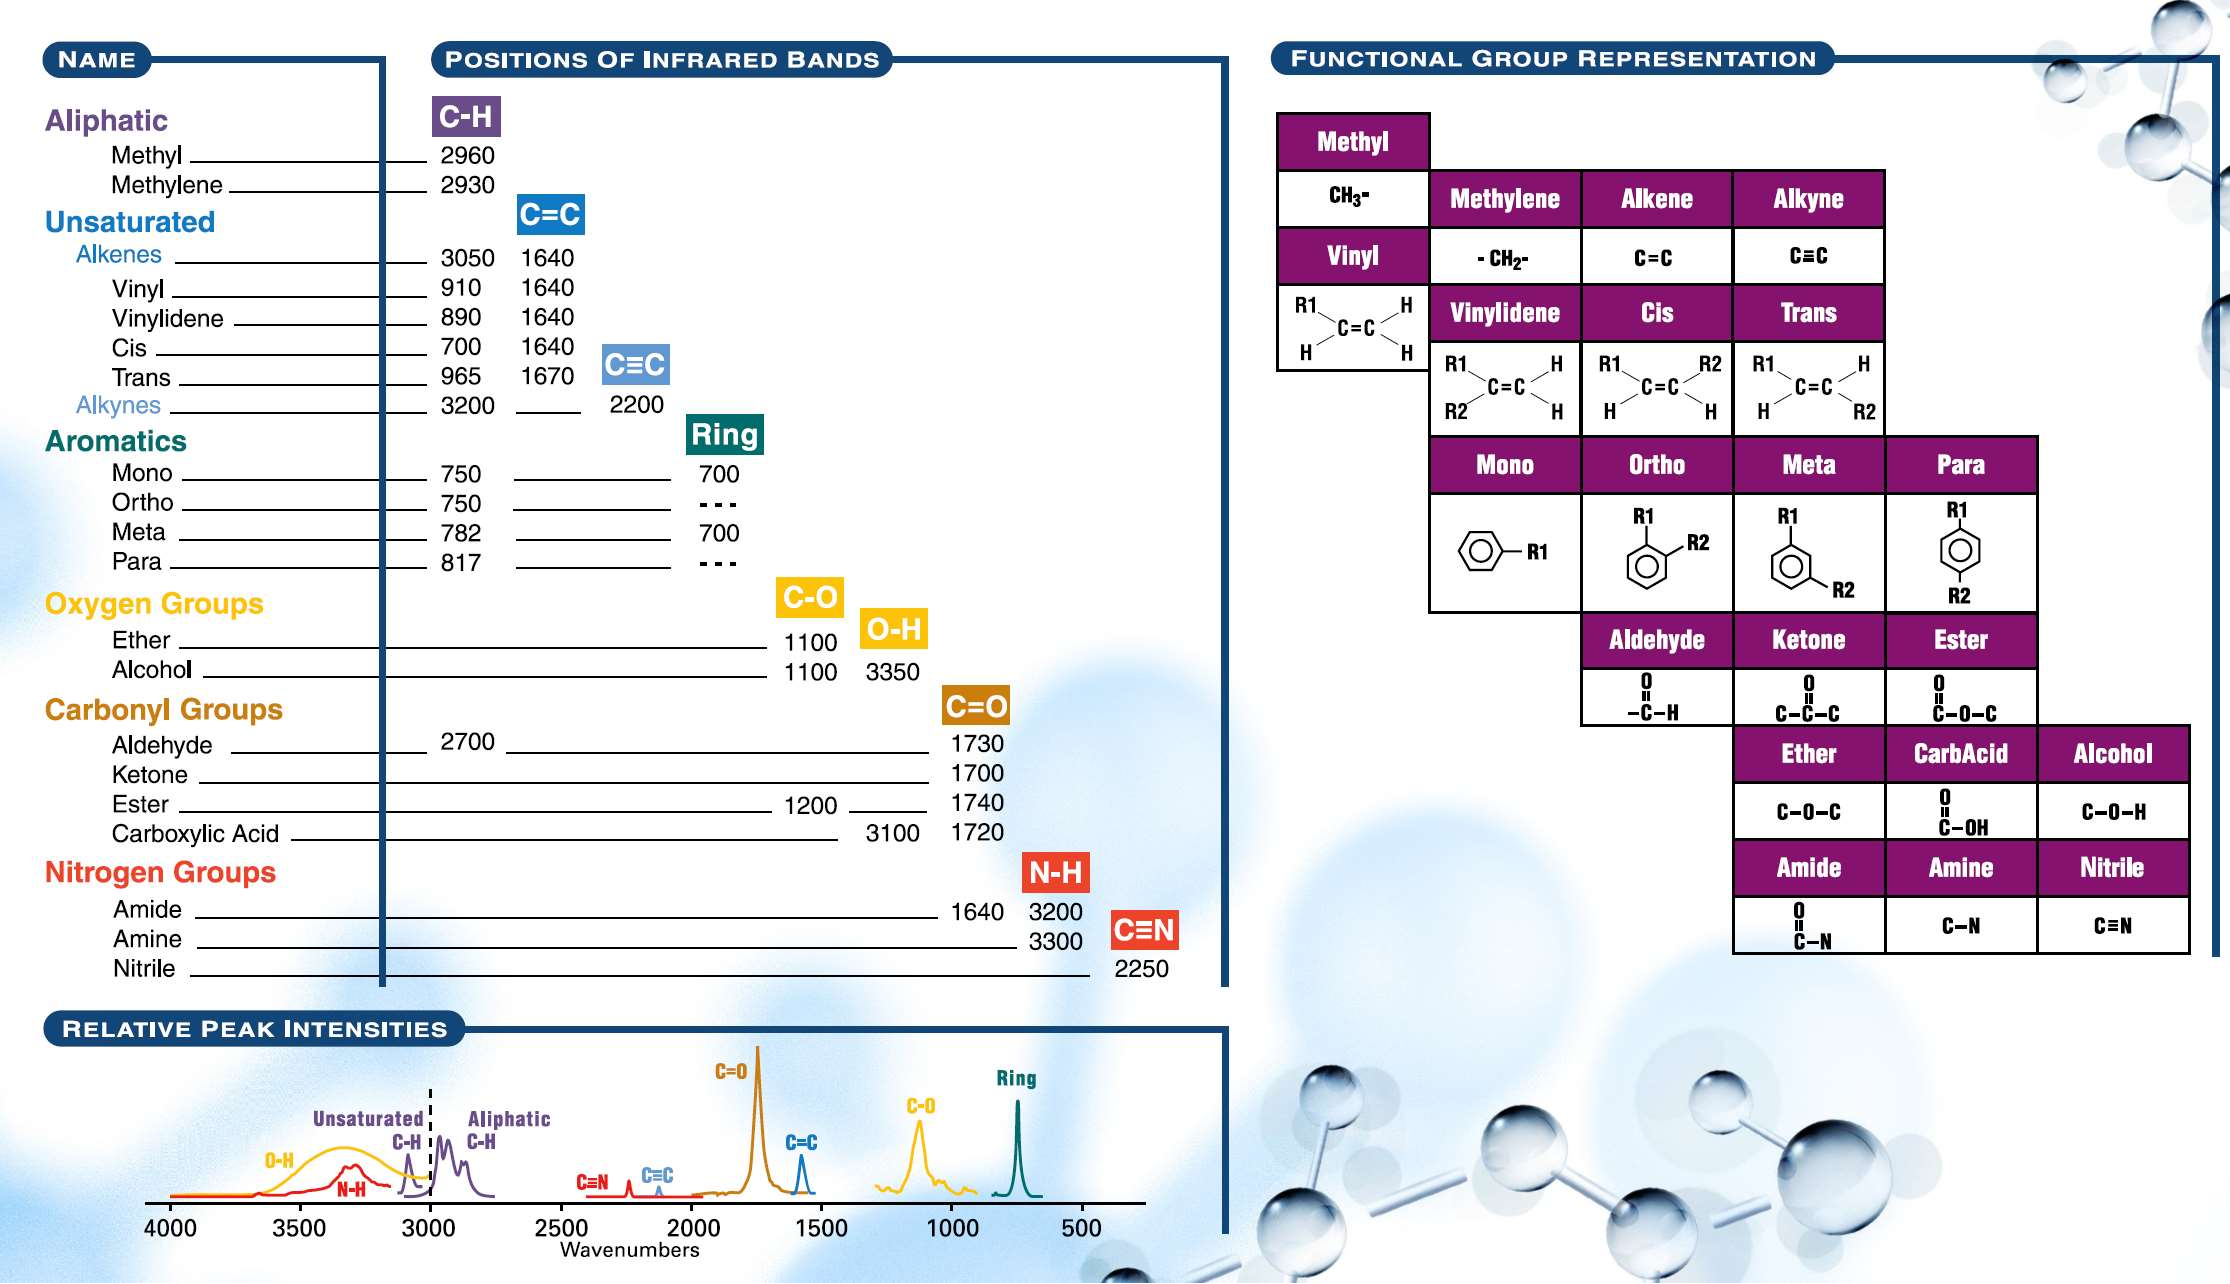
\includegraphics[width=0.809\paperwidth]{3_028}}
\endgroup

\vfill
